\section{\gls{DPR} for Internal Fault Mitigation}\label{InternalFaults}
\begin{figure}
    \centering
    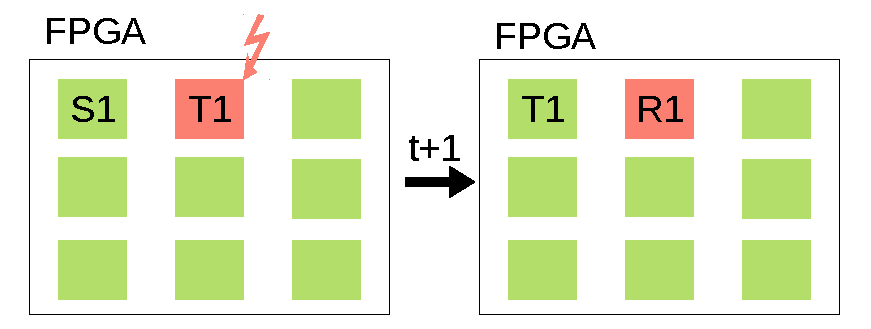
\includegraphics[width=\columnwidth]{graphics/faultyTile2.pdf}
    %\resizebox{\smallColumnWidth}{!}{\tikzset{every picture/.style={line width=0.25pt}} %set default line width to 0.75pt        

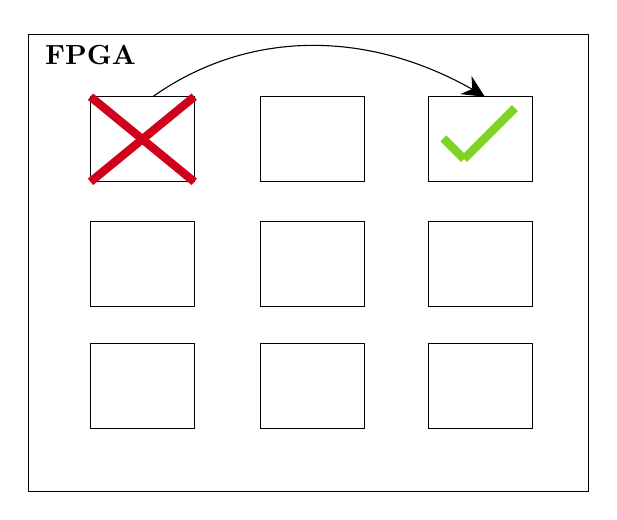
\begin{tikzpicture}[x=0.75pt,y=0.75pt,yscale=-1,xscale=1]
%uncomment if require: \path (0,279); %set diagram left start at 0, and has height of 279

%Shape: Rectangle [id:dp5787797491333819] 
\draw   (6,20) -- (276,20) -- (276,240) -- (6,240) -- cycle ;
%Shape: Rectangle [id:dp17505095690594463] 
\draw   (36,50) -- (86,50) -- (86,91) -- (36,91) -- cycle ;
%Shape: Rectangle [id:dp3058047377979807] 
\draw   (36,110) -- (86,110) -- (86,151) -- (36,151) -- cycle ;
%Shape: Rectangle [id:dp004684645465554249] 
\draw   (36,169) -- (86,169) -- (86,210) -- (36,210) -- cycle ;
%Shape: Rectangle [id:dp3077757040785931] 
\draw   (118,50) -- (168,50) -- (168,91) -- (118,91) -- cycle ;
%Shape: Rectangle [id:dp7450799349257811] 
\draw   (118,110) -- (168,110) -- (168,151) -- (118,151) -- cycle ;
%Shape: Rectangle [id:dp2725857150503048] 
\draw   (118,169) -- (168,169) -- (168,210) -- (118,210) -- cycle ;
%Shape: Rectangle [id:dp3816815123242099] 
\draw   (199,50) -- (249,50) -- (249,91) -- (199,91) -- cycle ;
%Shape: Rectangle [id:dp2885393682660524] 
\draw   (199,110) -- (249,110) -- (249,151) -- (199,151) -- cycle ;
%Shape: Rectangle [id:dp4969175268738504] 
\draw   (199,169) -- (249,169) -- (249,210) -- (199,210) -- cycle ;
%Straight Lines [id:da8580754234796655] 
\draw [color={rgb, 255:red, 208; green, 2; blue, 27 }  ,draw opacity=1 ][line width=3]    (36,50) -- (86,91) ;


%Straight Lines [id:da5772916268060835] 
\draw [color={rgb, 255:red, 208; green, 2; blue, 27 }  ,draw opacity=1 ][line width=3]    (86,50) -- (36,91) ;


%Curve Lines [id:da5702734861080319] 
\draw    (66,50) .. controls (112.04,17.33) and (171.3,17) .. (224.39,49.02) ;
\draw [shift={(226,50)}, rotate = 211.67000000000002] [fill={rgb, 255:red, 0; green, 0; blue, 0 }  ][line width=0.75]  [draw opacity=0] (10.72,-5.15) -- (0,0) -- (10.72,5.15) -- (7.12,0) -- cycle    ;

%Straight Lines [id:da7282259837027933] 
\draw [color={rgb, 255:red, 126; green, 211; blue, 33 }  ,draw opacity=1 ][line width=3]    (240.5,55.5) -- (216,80) ;


%Straight Lines [id:da7142424530641487] 
\draw [color={rgb, 255:red, 126; green, 211; blue, 33 }  ,draw opacity=1 ][line width=3]    (216,80) -- (206,70) ;



% Text Node
\draw (36,30) node  [align=left] {\textbf{FPGA}};


\end{tikzpicture}
}
    \caption{Internal Fault Mitigation - functionality from a faulty tile is moved to a healthy area with \gls{DPR}}\label{fig:internalFaultMitigation}
\end{figure}

%\tikzset{every picture/.style={line width=0.25pt}} %set default line width to 0.75pt        

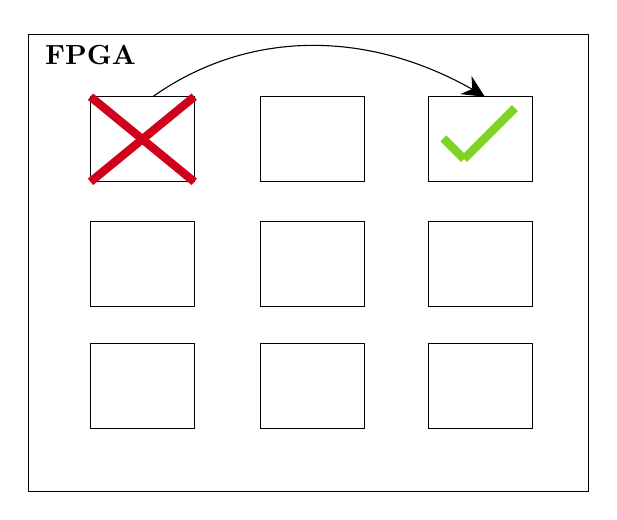
\begin{tikzpicture}[x=0.75pt,y=0.75pt,yscale=-1,xscale=1]
%uncomment if require: \path (0,279); %set diagram left start at 0, and has height of 279

%Shape: Rectangle [id:dp5787797491333819] 
\draw   (6,20) -- (276,20) -- (276,240) -- (6,240) -- cycle ;
%Shape: Rectangle [id:dp17505095690594463] 
\draw   (36,50) -- (86,50) -- (86,91) -- (36,91) -- cycle ;
%Shape: Rectangle [id:dp3058047377979807] 
\draw   (36,110) -- (86,110) -- (86,151) -- (36,151) -- cycle ;
%Shape: Rectangle [id:dp004684645465554249] 
\draw   (36,169) -- (86,169) -- (86,210) -- (36,210) -- cycle ;
%Shape: Rectangle [id:dp3077757040785931] 
\draw   (118,50) -- (168,50) -- (168,91) -- (118,91) -- cycle ;
%Shape: Rectangle [id:dp7450799349257811] 
\draw   (118,110) -- (168,110) -- (168,151) -- (118,151) -- cycle ;
%Shape: Rectangle [id:dp2725857150503048] 
\draw   (118,169) -- (168,169) -- (168,210) -- (118,210) -- cycle ;
%Shape: Rectangle [id:dp3816815123242099] 
\draw   (199,50) -- (249,50) -- (249,91) -- (199,91) -- cycle ;
%Shape: Rectangle [id:dp2885393682660524] 
\draw   (199,110) -- (249,110) -- (249,151) -- (199,151) -- cycle ;
%Shape: Rectangle [id:dp4969175268738504] 
\draw   (199,169) -- (249,169) -- (249,210) -- (199,210) -- cycle ;
%Straight Lines [id:da8580754234796655] 
\draw [color={rgb, 255:red, 208; green, 2; blue, 27 }  ,draw opacity=1 ][line width=3]    (36,50) -- (86,91) ;


%Straight Lines [id:da5772916268060835] 
\draw [color={rgb, 255:red, 208; green, 2; blue, 27 }  ,draw opacity=1 ][line width=3]    (86,50) -- (36,91) ;


%Curve Lines [id:da5702734861080319] 
\draw    (66,50) .. controls (112.04,17.33) and (171.3,17) .. (224.39,49.02) ;
\draw [shift={(226,50)}, rotate = 211.67000000000002] [fill={rgb, 255:red, 0; green, 0; blue, 0 }  ][line width=0.75]  [draw opacity=0] (10.72,-5.15) -- (0,0) -- (10.72,5.15) -- (7.12,0) -- cycle    ;

%Straight Lines [id:da7282259837027933] 
\draw [color={rgb, 255:red, 126; green, 211; blue, 33 }  ,draw opacity=1 ][line width=3]    (240.5,55.5) -- (216,80) ;


%Straight Lines [id:da7142424530641487] 
\draw [color={rgb, 255:red, 126; green, 211; blue, 33 }  ,draw opacity=1 ][line width=3]    (216,80) -- (206,70) ;



% Text Node
\draw (36,30) node  [align=left] {\textbf{FPGA}};


\end{tikzpicture}

\glspl{FPGA} provide high flexibility and good performance in many areas that require a high amount of concurrent computing and therefore benefit from a dedicated hardware implementation.
These properties prove useful for applications in the domain of aerospace and help to reduce the cost for satellites and spacecraft while providing high flexibility throughout the development process. 

But \glspl{FPGA} are especially vulnerable to cosmic radiation which can create a multitude of internal errors in the \gls{FPGA} and thereby breaking its intended functionality \cite{ito_total_2015}.
While there are radiation hardened \glspl{FPGA} available on the market, the mass of a space embedded system is still composed of 80\% radiation shielding \cite{ito_total_2015}.
Yet, this shielding is still not able to provide sufficient protection from radiation induced errors, especially on long term missions. 
Therefore, solutions for fault mitigation in aerospace \glspl{FPGA} need to be developed on the architectural level instead of the physical level. 
This may also provide the advantage of lower requirements for radiation shielding and therefore a reduced cost for payload on rocket launches.
Figure \ref{fig:internalFaultMitigation} depicts the basic concept of internal fault mitigation. 
An error occurs in Task 1 (\textit{T1}) and a healthy Spare Tile (\textit{S1}) is available. 
\textit{T1} is then moved to \textit{S1} in a partial-reconfiguration step and is ready for regular operation after the reconfiguration time \textit{t+1}.
A recovery of the tile Recovery 1 (\textit{R1}) is attempted and if it fails, it is marked as faulty for future reconfiguration operations.

The next section reviews the different types of faults and categorizes them. 

\subsection{Types of Internal Faults}
There are different types of faults that may occur in the lifetime of an \gls{FPGA}, a short overview over the most relevant ones is given in the following.
\par
\textbf{Transient Faults}
\begin{itemize}
    \item \glspl{SEU}, e.g. radiation induced \cite{alkady_fault-tolerant_2014}, \cite{lee_fault-tolerant_2017}
    \begin{itemize}
    \item Change of logic state in memory cell
    \item Commonly tackled by redundancy
    \item Built-in fault detection unit possible
    \end{itemize}
    \item Single Bit Errors (SBEs)
    \item Single Event Transients (SETs)
    \item Address Decoding Faults
\end{itemize}

Faults occur either in the interconnect of the \gls{FPGA} (which uses up to 80\% of the available silicon) or in its actual logic blocks \cite{alkady_fault-tolerant_2014}, \cite{jing_huang_routability_2004}.
\par
\textbf{Permanent Faults}
\begin{itemize}
    \item Time Dependant Dielectric Breakdowns (TDDBs)
    \item Electro Migration
    \item Hot Carrier Effect
\end{itemize}

Based on this review, two main categories of errors emerge.
Firstly, \textit{permanent faults} (also known as \textit{hard errors}), which include all faults that render the affected area completely unusable. 
Secondly, \textit{transient faults} (also known as \textit{soft errors}), which encompasses faults where a reclamation of the erroneous area may still be possible after the initial mitigation process.

To mitigate the aforementioned internal faults in an \gls{FPGA}, different strategies can be employed.
All of them feature \gls{DPR} as a means to move functional blocks from a faulty silicon area to a healthy one.
What sets them apart is the way of fault detection and the specifically employed \gls{DPR} strategy.

The following section introduces the general concept of a fault mitigation- and recovery flow. 

\subsection{Abstract Fault Mitigation Flow}\label{AbstractFaultMitigationFlow}
As the general scheme for fault mitigation is always the same, a brief introduction to the corner stones of every recovery flow is given (depicted in figure \ref{fig:internalFaultFlow}). 

\subsubsection{Detect Fault}
    One key aspect of fault mitigation is fault detection. 
    When faulty behaviour is detected, the origin of the fault needs to be determined.
    Generally, a dedicated (internal or external) control-unit is assigned to the task of result verification.
    This control-unit then gathers information about the location of the affected area and which functionality is corrupted.
\subsubsection{Mitigate Fault}
    After a successful isolation of the fault, steps towards its mitigation are taken.
    Due to external (e.g. increase in radiation) or internal (e.g. space, power) constraints, this stage may encompass some sort of estimation algorithm for the selection of a suitable \gls{PR} block.
    As a consequence, the system can dynamically adapt its fault resistance to changing circumstances.
\subsubsection{Resume Functionality}
    To fully leverage the advantage of \gls{DPR}, some sort of redundancy (e.g. \gls{TMR}) is usually employed.
    This allows the whole system to remain fully functional during the process of \gls{DPR} - the redundant modules will still provide the required data / processing during the reconfiguration. 
    The now freshly instantiated module then needs to re-sync its state with the rest of the system to return to its normal functionality.
\subsubsection{Recover Faulty Area}
    If a transient fault is responsible for the erroneous behaviour, the affected chip area may be recovered by error correction techniques like scrubbing \cite{reorda_error-detection_2017}. 
    In case of a successful recovery, the control-unit can mark the partition as healthy and reuse it at a later point in time.

\begin{center}
\begin{figure}[h]
    \centering
    \resizebox{\smallColumnWidth}{!} {
            \definecolor{one}{HTML}{E52B50}
    %\definecolor{two}{HTML}{fb8072}
    \definecolor{two}{HTML}{80b1d3}
\begin{tikzpicture}[]

\draw[solid]
(-2,0) node[fill=one!20,draw,rounded corners] (B) {Detect Fault}
(1,-1) node[fill=two!20,draw] (C) {Locate Affected Area}
(1,-2) node[fill=two!20,draw] (D) {Determine Affected Functionality}
(1,-3) node[fill=two!20,draw] (E) {Select Suitable PR Block}
(1,-4) node[fill=two!20,draw] (F) {Instantiate PR Block}
(1,-5) node[fill=one!20,draw] (G) {Resume Functionality}
(1,-6) node[fill=two!20,draw] (H) {Recover Faulty Area};
%\draw[dotted] (4, 2) -- (4,-3);
\draw[->, to path={-| (\tikztotarget)}] (B) edge (C);
\draw[->] (C) edge (D);
\draw[->] (D) edge (E);
\draw[->] (E) edge (F);
\draw[->] (F) edge (G);
\draw[->] (G) edge (H);
%\draw[->, to path={-| (\tikztotarget)}] (D) edge (E);
%\draw[->] (E) edge (F);
%\draw[->, to path={-| (\tikztotarget)}] (F) edge (G);
%\draw[->] (G) edge (H);
%\draw[->, to path={-| (\tikztotarget)}] (F) edge (G);
%\draw[->, to path={-| (\tikztotarget)}] (G) edge (H);
%\draw[->, to path={-| (\tikztotarget)}] (H) edge (A);
\draw[->, to path={-| (\tikztotarget)}] (G) edge (B);
\draw[->, to path={-| (\tikztotarget)}] (H) edge (B);
\end{tikzpicture}

    }
\caption{Abstract Fault Mitigation Flow}
\label{fig:internalFaultFlow}
\end{figure}
\end{center}

Each stage of this flow can be implemented with different architectural design choices.
These choices are influenced by available resources, real-time constraints and the desire of more control over the system behaviour.
The next sections introduce different architectures for a system that wants to utilize \gls{DPR} for fault mitigation.

\subsection{Spare Tile Architecture for \gls{DPR}}
This approach is taken in the work of \cite{lameres_radsat_nodate} and is extended in \cite{wilson_hybrid_2017}.
It creates a computer system that exhibits a higher fault tolerance against radiation induced faults while using only commercially available off-the-shelf \glspl{FPGA}. 
To achieve this, the computing system is designed as a \gls{PR} partition from the beginning (figure \ref{fig:SpareTileArchitecture}). 
\gls{TMR} with a voter is used to assess the correctness of the output. 
When one module fails to compute the expected result (i.e. the result of the other two modules), a partial reconfiguration flow is triggered.
One of the healthy spare tiles is selected for the instantiation of another compute module.
The usage of the scrubbing technique allows the eventual recovery of the faulty tile which decreases the likelihood of resource exhaustion. 
Scrubbing is also used to check the health of inactive tiles in intervals, so that the healthiness of the backup tiles is known at all time. 
An advantage of this approach is that all relevant computations can still be carried out by the two remaining healthy modules during the recovery process. 
It also increases the robustness of the system in comparison to a stand-alone \gls{TMR} + scrubbing approach.
The system has been verified theoretically by a Markov model, as well as in a real world scenario where the test system was exposed to a defined dose of radiation over a time-period (The \gls{MTBF} was increased by a factor of 90 in this test).

A system like this is easy to implement and creates a low resource overhead during the development phase while it provides drastically improved reliability.
The verification of the results in the voter and the selection of a healthy healthy spare tile for reconfiguration don't pose a significant computational load on the system.
As instantiation of a spare module is way faster than scrubbing a faulty tile (1ms vs 100ms), the chance of losing 2 active compute tiles in a short time frame is reduced. 
But as the complexity of such a design increases, the tile size also increases. 
This implies an increased overall area cost for the spare tiles on the \gls{FPGA} which makes efficient placement more difficult.
It also reduces the amount of available space for other desired functionalities. 

The work of \cite{martins_tmr_2015} follows a similar principle, but tries to optimize the tooling that is required for partial bitstream generation.
The goal of these optimizations is to reduce the overall resource waste by the provision of only one partial bitstream per module for all \textit{N} \glspl{RP}. %The following part could still be extended with more details 
Usual \gls{DPR} workflows require a dedicated partial bitstream for each \gls{RP}, which results in \textit{N} partial bitstreams for \textit{N} desired \gls{RP}.
\cite{martins_dynamic_2018} improves the previous work in \cite{martins_tmr_2015} and demonstrates its functionality in a scenario where permanent faults due to ageing are detected and mitigated.

\begin{center}
\begin{figure}[h]
    \centering
    \resizebox{\smallColumnWidth}{!} {
        \begin{tikzpicture}[]

\draw[solid]

(0,2) node[fill=cBlue!40,draw, minimum height=1.5cm, minimum width=2.5cm] (ASV) {\textbf{Voter / Control}}
(-3,0) node[fill=cYellow!60,draw, minimum height=1.5cm, minimum width=2.5cm] (AS) {Compute Tile}
(0,0) node[fill=cYellow!60,draw, minimum height=1.5cm, minimum width=2.5cm] (AM) {Compute Tile}
(3,0) node[fill=cYellow!60,draw, minimum height=1.5cm, minimum width=2.5cm] (AE) {Compute Tile}
(-3,-2) node[fill=cGreen!60,draw, minimum height=1.5cm, minimum width=2.5cm] (ASS) {Spare Tile}
(0,-2) node[fill=cGreen!60,draw, minimum height=1.5cm, minimum width=2.5cm] (AMS) {Spare Tile}
(3,-2) node[fill=cGreen!60,draw, minimum height=1.5cm, minimum width=2.5cm] (AES) {Spare Tile};

\draw[solid] (-4.5,3) rectangle (4.5,-3);

\end{tikzpicture}


    }
\caption{Spare Tile Architecture}
\label{fig:SpareTileArchitecture}
\end{figure}
\end{center}

\subsection{Task Based Architecture for \gls{DPR}}
If a more complex or diverse set of tasks needs to be processed, a task based architecture may be used. 
This usually includes the usage of some kind of \gls{RTOS} with a scheduler.
The scheduler is extended with a placer component which computes the optimal location of a hardware accelerated task in the \gls{RP}.
To make a heterogeneous set of tasks possible, all tasks can share the same memory interface and interact with the \gls{RTOS} over a memory map, as shown in \cite{wang_dynamic_2018} (see also figure \ref{fig:TaskBased}).

\begin{figure}
    \centering
    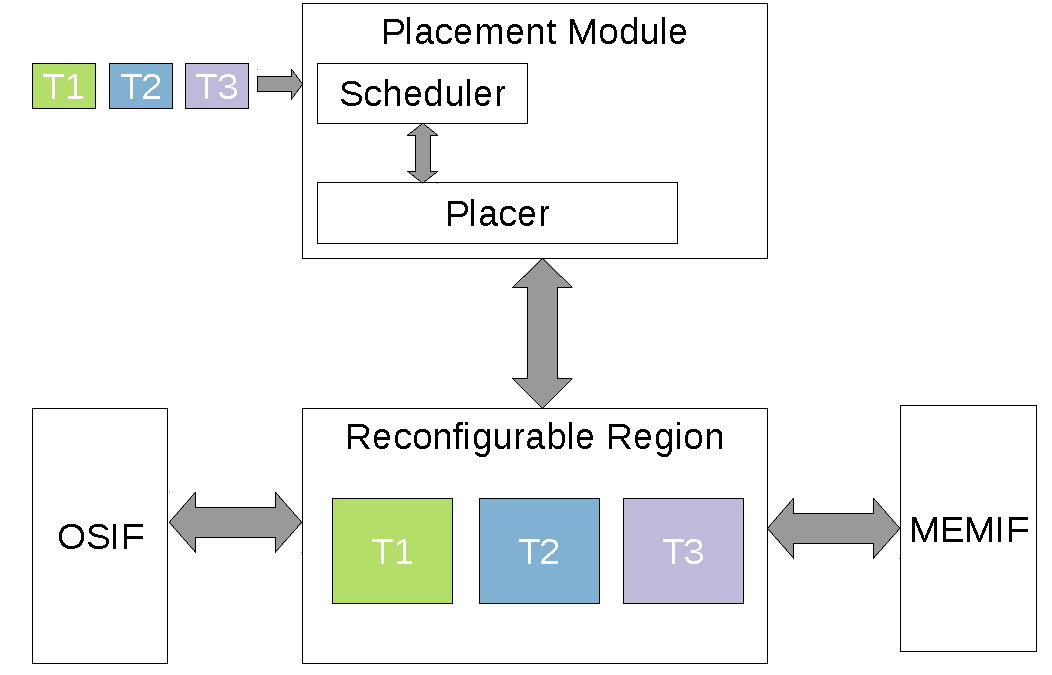
\includegraphics[width=\columnwidth]{graphics/TaskBased.pdf}
    %\resizebox{\smallColumnWidth}{!}{\tikzset{every picture/.style={line width=0.25pt}} %set default line width to 0.75pt        

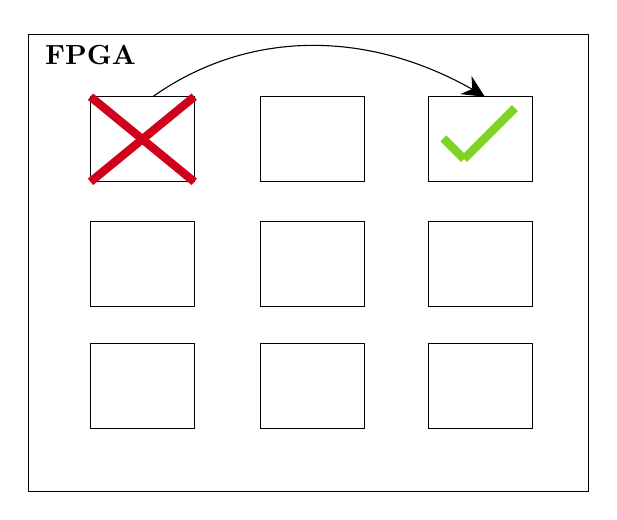
\begin{tikzpicture}[x=0.75pt,y=0.75pt,yscale=-1,xscale=1]
%uncomment if require: \path (0,279); %set diagram left start at 0, and has height of 279

%Shape: Rectangle [id:dp5787797491333819] 
\draw   (6,20) -- (276,20) -- (276,240) -- (6,240) -- cycle ;
%Shape: Rectangle [id:dp17505095690594463] 
\draw   (36,50) -- (86,50) -- (86,91) -- (36,91) -- cycle ;
%Shape: Rectangle [id:dp3058047377979807] 
\draw   (36,110) -- (86,110) -- (86,151) -- (36,151) -- cycle ;
%Shape: Rectangle [id:dp004684645465554249] 
\draw   (36,169) -- (86,169) -- (86,210) -- (36,210) -- cycle ;
%Shape: Rectangle [id:dp3077757040785931] 
\draw   (118,50) -- (168,50) -- (168,91) -- (118,91) -- cycle ;
%Shape: Rectangle [id:dp7450799349257811] 
\draw   (118,110) -- (168,110) -- (168,151) -- (118,151) -- cycle ;
%Shape: Rectangle [id:dp2725857150503048] 
\draw   (118,169) -- (168,169) -- (168,210) -- (118,210) -- cycle ;
%Shape: Rectangle [id:dp3816815123242099] 
\draw   (199,50) -- (249,50) -- (249,91) -- (199,91) -- cycle ;
%Shape: Rectangle [id:dp2885393682660524] 
\draw   (199,110) -- (249,110) -- (249,151) -- (199,151) -- cycle ;
%Shape: Rectangle [id:dp4969175268738504] 
\draw   (199,169) -- (249,169) -- (249,210) -- (199,210) -- cycle ;
%Straight Lines [id:da8580754234796655] 
\draw [color={rgb, 255:red, 208; green, 2; blue, 27 }  ,draw opacity=1 ][line width=3]    (36,50) -- (86,91) ;


%Straight Lines [id:da5772916268060835] 
\draw [color={rgb, 255:red, 208; green, 2; blue, 27 }  ,draw opacity=1 ][line width=3]    (86,50) -- (36,91) ;


%Curve Lines [id:da5702734861080319] 
\draw    (66,50) .. controls (112.04,17.33) and (171.3,17) .. (224.39,49.02) ;
\draw [shift={(226,50)}, rotate = 211.67000000000002] [fill={rgb, 255:red, 0; green, 0; blue, 0 }  ][line width=0.75]  [draw opacity=0] (10.72,-5.15) -- (0,0) -- (10.72,5.15) -- (7.12,0) -- cycle    ;

%Straight Lines [id:da7282259837027933] 
\draw [color={rgb, 255:red, 126; green, 211; blue, 33 }  ,draw opacity=1 ][line width=3]    (240.5,55.5) -- (216,80) ;


%Straight Lines [id:da7142424530641487] 
\draw [color={rgb, 255:red, 126; green, 211; blue, 33 }  ,draw opacity=1 ][line width=3]    (216,80) -- (206,70) ;



% Text Node
\draw (36,30) node  [align=left] {\textbf{FPGA}};


\end{tikzpicture}
}
    \caption{Task Based Architecture with a memory map for a unified communication interface}\label{fig:TaskBased}
\end{figure}

The work in \cite{sharma_run-time_2018} proposes not only ways for fault recovery, but also ways of maintaining as much functionality as possible under varying power constraints. 
\gls{DPR} is utilized to achieve \gls{RT-SA}, i.e. a system that can dynamically alter its architecture to mitigate the effect of changed circumstances.

\cite{wang_dynamic_2018}

\section{\gls{DPR} in \glspl{NoC}}
Introduced by \cite{wehbe_secure_2016}.
\subsection{\gls{DPR} for increased security}
\subsection{\gls{DPR} for failed routers}

